\chapter{Lecture 7: Topics in String Theory}

These notes follow Leonard Susskind's seventh lecture in the supplementary Winter 2011 string-theory track of \emph{Cosmology and Black Holes}, curated by LazyingArt LLC. The lecture resumes an unfinished question about black-hole entropy rather than starting from scratch. Susskind first assembles a short list of simple equations, then uses them to relate long strings to black holes, broadens the lesson into the holographic principle, and finally pivots to the metric of an expanding universe and the exponentially growing de Sitter solution.

\section{Setup and the Target Problem}

The lecture opens as a continuation of the previous discussion. Susskind first answers a leftover counting question: identical small strings are treated as indistinguishable when they have the same length, but their positions inside the box are still counted. That brief exchange matters because the entire lecture remains tied to the earlier long-string counting problem.

He then states the real goal. The derivation he has in mind is intentionally indirect. It is supposed to be mathematically simple, almost embarrassingly simple, but conceptually subtle. The strategy is to put a few scale-setting equations on the board first, and only then compare string theory with black-hole thermodynamics.

\section{Natural Units and the Relevant Scales}

Susskind begins by fixing units,
\begin{equation}
c=\hbar=1,
\end{equation}
while deliberately leaving Newton's constant unfixed. In these units space and time are measured in the same units, and the point of the opening warm-up is to identify the dimensions of mass and of \(G_N\).

\begin{figure}
\centering

\includegraphics[width=0.56\textwidth]{lecture_07_figure_02.png}
\caption{Natural-units setup for the energy relation. At this stage the board visibly carries only \(c=\hbar=1\) and the opening symbol \(E\); the equations written below are the cleaned reconstruction of the intended dimensional argument.}
\end{figure}

The board at this moment is still almost empty, so the transcript has to carry the mathematics. The intended dimensional chain is
\begin{align}
E &\sim \frac{\hbar c}{\lambda}, \\
m &= \frac{E}{c^2},
\end{align}
and therefore, once \(c=\hbar=1\),
\begin{equation}
m \sim \frac{1}{\lambda}.
\end{equation}
So mass has the dimensions of inverse length.

\begin{remark}
The spoken discussion around \(E=mc^2\) is partly joking and verbally garbled. The mathematical point is only that in natural units mass and inverse length carry the same dimensions.
\end{remark}

The next step is to determine the dimensions of Newton's constant from the simplest equation that contains it:
\begin{equation}
a \sim \frac{G_N M}{R^2}.
\end{equation}
In the chosen units,
\[
[a] \sim \frac{L}{T^2} \sim \frac{1}{L}, \qquad [M] \sim \frac{1}{L}, \qquad [R^2]\sim L^2.
\]
Therefore \(G_N\) must have dimensions of area:
\begin{equation}
[G_N]=L^2.
\end{equation}
The cleaned form of the lecture's statement is thus
\begin{equation}
G_N=\ell_p^2,
\end{equation}
namely Newton's constant is the Planck area.

This is immediately useful for black holes, because the Bekenstein-Hawking entropy will later be area measured in Planck units. But Susskind next turns from gravity in general to gravity in string theory. The force of gravity is represented by a cartoon of graviton exchange, and the important lesson of the cartoon is only this: emission and absorption each contribute one power of the string coupling, so gravitational strength is proportional to \(g_s^2\). Since \(g_s\) is dimensionless, a length scale must supply the missing area dimensions. The only available length on the string side is \(\ell_s\). Hence
\begin{equation}
G_N \sim g_s^2 \ell_s^2,
\end{equation}
or equivalently
\begin{equation}
\ell_p \sim g_s \ell_s.
\end{equation}

This is the first bridge between the two columns of the lecture: the Planck scale on the gravity side and the string scale on the string side are not independent.

\section{Long Strings as Random Walks}

Only after the scales are in place does Susskind turn to entropy on the string side. The key picture is a highly excited long string treated as a random walk on a lattice. At each new vertex the string makes one of a few discrete choices. The exact combinatorial base is not the point. What matters is that the number of elementary decisions is proportional to the number of steps.

\begin{figure}
\centering

\includegraphics[width=0.42\textwidth]{lecture_07_figure_03.png}

\vspace{1em}

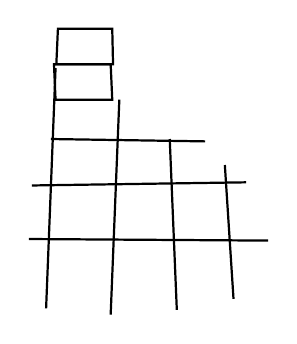
\begin{tikzpicture}[x=1cm,y=1cm]
\draw[line width=0.8pt] (-0.10,-0.10) -- (0.02,2.95);
\draw[line width=0.8pt] (0.72,-0.18) -- (0.83,2.55);
\draw[line width=0.8pt] (1.56,-0.12) -- (1.47,2.05);
\draw[line width=0.8pt] (2.28,0.02) -- (2.17,1.72);

\draw[line width=0.8pt] (-0.32,0.78) -- (2.72,0.76);
\draw[line width=0.8pt] (-0.28,1.46) -- (2.44,1.50);
\draw[line width=0.8pt] (-0.04,2.05) -- (1.92,2.02);

\draw[line width=0.8pt] (0.02,2.55) -- (0.74,2.55) -- (0.72,3.00) -- (0.00,3.00) -- cycle;
\draw[line width=0.8pt] (0.03,3.00) -- (0.75,3.00) -- (0.74,3.45) -- (0.05,3.45) -- cycle;
\end{tikzpicture}
\caption{Rough lattice sketch for the string random walk. The screenshot preserves the original board evidence, while the redraw keeps only the discrete, uneven, step-wise character of the picture rather than claiming an exact combinatorial construction.}
\end{figure}

The lecture's entropy formula is therefore a counting formula. If \(L\) is the total length of the long string and \(\ell_s\) is the elementary step size, then the number of steps is \(L/\ell_s\), so
\begin{equation}
S_{\mathrm{str}} \sim \frac{L}{\ell_s}.
\end{equation}
This is the point of the random-walk picture: entropy is not just ``proportional to length'' in a vague sense; it is the number of elementary decisions along the walk.

The mass of the string is handled in the same discrete spirit. One elementary segment has length \(\ell_s\), and since mass scales as inverse length,
\begin{equation}
m_{\mathrm{seg}} \sim \frac{1}{\ell_s}.
\end{equation}
The total string contains \(L/\ell_s\) such segments, so
\begin{equation}
M \sim \frac{L}{\ell_s}\,m_{\mathrm{seg}} \sim \frac{L}{\ell_s^2}.
\end{equation}
Rearranging,
\begin{equation}
L \sim M\ell_s^2.
\end{equation}
Substituting this into the entropy formula gives the compact string-side relation that Susskind wants on the board:
\begin{equation}
S_{\mathrm{str}} \sim M\ell_s.
\end{equation}

The lecture briefly notes that treating the total mass as the sum of elementary segment masses is a mild oversimplification, but good enough for the scaling argument. The point is not a refined string spectrum; it is a reliable parametric relation between entropy and mass.

\section{First Comparison with Black-Hole Entropy}

At this stage the lecture has assembled a string-theory column and is ready to place it next to black-hole physics.

\begin{figure}
\centering

\includegraphics[width=0.56\textwidth]{lecture_07_figure_04.png}
\caption{String-side equations before the black-hole comparison. The lower mass relation is partly hidden on the board, but the surrounding derivation fixes its clean form as \(M \sim L/\ell_s^2\).}
\end{figure}

The board organization on the string side can be written in cleaned scaling form as
\begin{align}
\ell_p &\sim g_s \ell_s, \\
S_{\mathrm{str}} &\sim \frac{L}{\ell_s} \sim M\ell_s, \\
M &\sim \frac{L}{\ell_s^2}.
\end{align}
This is precisely the set of formulas Susskind wants visible before moving to the black-hole column.

The black-hole side begins with the Bekenstein-Hawking formula,
\begin{equation}
S_{\mathrm{BH}}=\frac{A}{4G_N}.
\end{equation}
For the lecture's scaling argument, the coefficient \(1/4\) is temporarily set aside. Using the Schwarzschild scaling
\begin{equation}
R_s \sim M G_N,
\end{equation}
one has
\begin{equation}
A \sim R_s^2 \sim M^2 G_N^2,
\end{equation}
and so
\begin{equation}
S_{\mathrm{BH}} \sim \frac{A}{G_N} \sim M^2 G_N \sim M^2 \ell_p^2.
\end{equation}

This is where the lecture deliberately lingers. The comparison is suggestive but not an identity:
\[
S_{\mathrm{str}} \sim M\ell_s,
\qquad
S_{\mathrm{BH}} \sim M^2\ell_p^2.
\]
Both are entropy formulas. Both involve mass multiplied by a length scale in some power. But they are not the same formula, and Susskind insists on that difference rather than hiding it.

The naive mistake would be to imagine that a black hole is ``just a string'' and therefore should satisfy the free long-string entropy law. What is missing is the effect of self-gravity. A gravitating object is not a gas placed in a box whose size was chosen independently; gravitational attraction changes the size, the energy, and therefore the entropy-energy relation. That is why a direct identification of the two formulas is the wrong idea.

\section{Adiabatic String--Black-Hole Correspondence}

What replaces the naive identification is a reversible thought experiment. In string theory the coupling \(g_s\) can be varied. If \(g_s\) is made very small, gravity effectively turns off and a highly excited object behaves like a long string. If \(g_s\) is increased, gravity becomes stronger and can collapse such a string into a black hole. The lecture asks for the inverse process: start with a black hole and slowly turn the coupling down.

The word ``slowly'' is essential. Entropy is taken to be an adiabatic invariant, so varying the coupling adiabatically does not change the entropy. The mass, however, does change, because lowering the coupling removes negative gravitational binding energy and lets the total mass rise.

Susskind also emphasizes a second ingredient. Before any detailed formula for black-hole entropy is used, the only dimensionless combination available on the black-hole side is \(M\ell_p\). At fixed \(\ell_s\), and using \(\ell_p \sim g_s\ell_s\), the relevant isentropic curve is therefore characterized by
\begin{equation}
M g_s = M_0 g_{s,0},
\end{equation}
where \(M_0\) and \(g_{s,0}\) refer to the original black hole we are trying to understand.

The second curve in parameter space is the crossover curve between black-hole behavior and string behavior. The heuristic criterion is that the Schwarzschild radius should become comparable to the string scale:
\begin{equation}
R_s \sim \ell_s.
\end{equation}
Using \(R_s \sim M G_N\) together with \(G_N \sim g_s^2\ell_s^2\), this becomes
\begin{equation}
M G_N \sim \ell_s
\qquad \Longrightarrow \qquad
M g_s^2 \sim \frac{1}{\ell_s}.
\end{equation}

\paragraph{Worked derivation of the crossover scaling.}
Let \((M_\ast,g_{s,\ast})\) denote the point where the adiabat meets the crossover curve. Then
\begin{align}
M_\ast g_{s,\ast} &= M_0 g_{s,0}, \\
M_\ast g_{s,\ast}^2 &\sim \frac{1}{\ell_s}.
\end{align}
From the first equation,
\begin{equation}
g_{s,\ast}=\frac{M_0 g_{s,0}}{M_\ast}.
\end{equation}
Substituting into the second gives
\begin{equation}
M_\ast \left(\frac{M_0 g_{s,0}}{M_\ast}\right)^2 \sim \frac{1}{\ell_s},
\end{equation}
so
\begin{equation}
M_\ast \ell_s \sim M_0^2 g_{s,0}^2 \ell_s^2.
\end{equation}
Using \(G_{N,0}\sim g_{s,0}^2\ell_s^2\), this becomes
\begin{equation}
M_\ast \ell_s \sim M_0^2 G_{N,0}.
\end{equation}

But at the crossover point the object has become string-like, and the string entropy formula applies:
\begin{equation}
S_{\mathrm{str},\ast} \sim M_\ast \ell_s.
\end{equation}
Since entropy was unchanged along the adiabatic path, this is also the entropy of the original black hole:
\begin{equation}
S_{\mathrm{BH}}(M_0) \sim M_0^2 G_{N,0} \sim M_0^2 \ell_{p,0}^2.
\end{equation}
This is the payoff of the lecture. One does not derive the black-hole entropy formula by treating the original black hole as a free string. One slowly follows the black hole until it becomes string-like, reads off the entropy there, and transports that answer back along an adiabat.

What this explains is the scaling. What it does \emph{not} explain is the exact numerical coefficient \(1/4\). Susskind is careful about this. The crossover is not sharply defined, and the argument is only parametric. More refined supersymmetric calculations can recover the exact coefficient in special settings, but conceptually the crucial point is already here: black-hole entropy behaves as though black holes possess microscopic degrees of freedom.

The lecture then steps back and states the historical lesson. If the calculation had produced a volume law such as \(M^3\ell_p^3\), it would have suggested ordinary bulk counting. Instead it reproduces an area law. That does not make black holes less strange. It sharpens the puzzle by showing that the microscopic interpretation really is encoded in area rather than volume.

\section{Maximum Entropy and the Holographic Principle}

From here the lecture changes question. The new question is no longer ``What is the entropy of a black hole?'' but ``What is the maximum entropy that any region can contain?''

Susskind first reconstructs the ordinary volume-counting intuition. Divide a room into cells, one yes-no question per cell: occupied or empty. Then the number of configurations is
\begin{equation}
\Omega = 2^N,
\qquad
N \sim \frac{V}{V_{\mathrm{cell}}},
\end{equation}
and so the maximal entropy in such a toy model is
\begin{equation}
S_{\max}=\log \Omega \sim \frac{V}{V_{\mathrm{cell}}}\log 2.
\end{equation}
This is the familiar expectation that maximum entropy scales with volume, because the number of local degrees of freedom scales with volume.

Gravity changes the conclusion. Consider a spatial region with boundary area \(A\), containing some matter with entropy \(S_{\mathrm{initial}}\) and total mass below the threshold for already being a black hole of that size. Now add an incoming shell carrying just enough extra mass to make the whole configuration collapse into a black hole that exactly fills the region. The material of the shell does not matter; the only point is its mass.

The final state has entropy
\begin{equation}
S_{\mathrm{final}}=\frac{A}{4G_N}.
\end{equation}
By the second law,
\begin{equation}
S_{\mathrm{initial}} \le S_{\mathrm{final}}.
\end{equation}
Therefore no configuration that fits inside the region can have more entropy than the black hole that just fills it. The lecture's conclusion is
\begin{equation}
S_{\max}=\frac{A}{4G_N},
\end{equation}
or, more cautiously as a bound,
\begin{equation}
S \le \frac{A}{4G_N}.
\end{equation}

\begin{definition}
The holographic principle is the statement that the independent degrees of freedom of a gravitating region are bounded by the area of its boundary measured in Planck units, not by its volume. Equivalently, one may think of the boundary as carrying at most one degree of freedom per Planck area.
\end{definition}

This is the second major conceptual payoff of the lecture. Ordinary local reasoning suggests that independent variations at many interior points should lead to a volume law. Gravity instead imposes an area law. The difference is not small; for a macroscopic region, the number of Planck cells on the boundary is vastly smaller than the number in the volume.

\section{The Cosmology Pivot}

A question from the room now redirects the lecture toward cosmology. Susskind explicitly says that he will not derive Einstein's equations here; he will simply write down the relevant class of solutions. The chosen case is the spatially flat universe, so the metric is
\begin{equation}
ds^2=-dt^2+a(t)^2\,dx_i dx_i,
\qquad
dx_i dx_i = dx^2+dy^2+dz^2.
\end{equation}
The function \(a(t)\) is the scale factor. It is the only source of time dependence in the spatial geometry.

If two galaxies remain at fixed coordinate separation \(\Delta x\), their proper distance is
\begin{equation}
d(t)=a(t)\,\Delta x.
\end{equation}
Differentiating with respect to time gives
\begin{equation}
v=\dot d=\Delta x\,\dot a=\frac{\dot a}{a}\,d.
\end{equation}
This motivates the definition
\begin{equation}
H=\frac{\dot a}{a},
\end{equation}
so that
\begin{equation}
v=Hd.
\end{equation}
This is Hubble's law in the lecture's form.

Susskind pauses to stress a subtle point that is easy to lose in cleaned notes: this formula is an equal-time relation. It tells us the relation between proper distance and recession speed at a single instant of cosmological time. It is not yet the full observational formula for what one actually sees when looking at a distant galaxy along the past light cone.

He then draws out a consequence of the formula. In units with \(c=1\), the distance at which recession speed reaches the speed of light is
\begin{equation}
d_H \sim \frac{1}{H}.
\end{equation}
Objects farther away can recede faster than light without violating local special relativity, because nothing is locally passing through anything else faster than light; rather, the intervening geometry is stretching.

The lecture next isolates the case most relevant for the next meeting: the Hubble parameter tends to a true constant. Then
\begin{equation}
\dot a = Ha,
\end{equation}
whose solution is
\begin{equation}
a(t)=a_0 e^{Ht}.
\end{equation}
Thus the scale factor grows exponentially, and so do proper distances between fixed-coordinate points.

\begin{remark}
Susskind briefly speaks of an exponential with \(2Ht\) when referring to the spatial metric coefficient. The scale factor itself is \(a(t)=a_0e^{Ht}\); therefore the coefficient \(a(t)^2\) appearing in the metric grows as \(e^{2Ht}\).
\end{remark}

A universe with this behavior is de Sitter space. The lecture stops here on purpose. The next step, deferred to the next lecture, is that de Sitter space has a horizon, in a sense complementary to the horizon of a black hole.

\section{Summary}

The lecture's structure is unusually clean. First come the scale-setting equations: in natural units mass is inverse length, Newton's constant is an area, and string theory relates the Planck and string scales by \(G_N \sim g_s^2\ell_s^2\). Next comes the long-string counting argument, which gives \(S_{\mathrm{str}} \sim M\ell_s\). Only then does Susskind place that formula beside \(S_{\mathrm{BH}} \sim M^2\ell_p^2\), reject the naive identification, and replace it with the adiabatic string--black-hole correspondence.

The result is not an exact derivation of \(A/(4G_N)\), but a parametric explanation for why black-hole entropy scales the way it does and why it should be read as evidence for microscopic structure. From there the lecture widens the lesson into the holographic bound \(S_{\max}\le A/(4G_N)\), and ends by shifting to cosmology: the flat FRW metric, Hubble's law, the horizon scale \(1/H\), and the exponential expansion \(a(t)=a_0e^{Ht}\) that defines de Sitter space.